\chapter{Theory}
This chapter contains the theoretical foundations necessary to understand parts of this thesis. 
The signal processing and neural network preliminaries will be explained.
Further the problem formulations will be represented in a mathematical viewpoint.

%The problems will be described in a mathematical way and each solution concept explained so that it can be understood.

% sp
% --
% signal processing

\section{Signal Processing and Feature Extraction}\label{sec:features}
This section describes how raw waveforms from audio files are processed and what meaningfull features can be extracted from them.
\subsection{Raw Audio Waveforms}\label{sec:raw_audio}
Physical acoustic waves are recorded by microphones, translating mechanincal vibrations to electrical signals, which can be stored to waveform files.
The Focus is here only on the raw waveform files and its data.
First it is to mention that waveform files are stored in some kind of audio format, e.g. .wav files, using parameters such as bit resolution, e.g. 32 bit floating point, and most importantly a sample rates $f_s$. 
The sample rate tells, which frequency range of the continuous acoustic waves form is possible to store in a discrete representation.
This is restricted by the Nyquist-Shannon sampling theorem, where the maximal frequency of the signal should not be larger than the half of the sampling frequency, otherwise aliasing effects occur. 
Thats why a usual CD format has a sampling frequency of 44.1kHz resulting in a maximum frequency of 22.05kHz, and usually humans do not hear above 20kHz frequencies.
However it is also possible to go far beyong those 44.1kHz, as it is used in telephone systems with a sampling rate of 8kHz.
This is because, voice does not need that high sampling frequency to be understandable and with enough quality.
The audio files of the speech command dataset are recorded with a sampling rate of 16kHz, which is totally enough for human speech.
Further those audio files in the speech command dataset have a time length of 1s.
The author recorded his own speech commands with one example of each command shown in \rfig{raw_audio_my}.

\begin{figure}[!ht]
  \centering
    %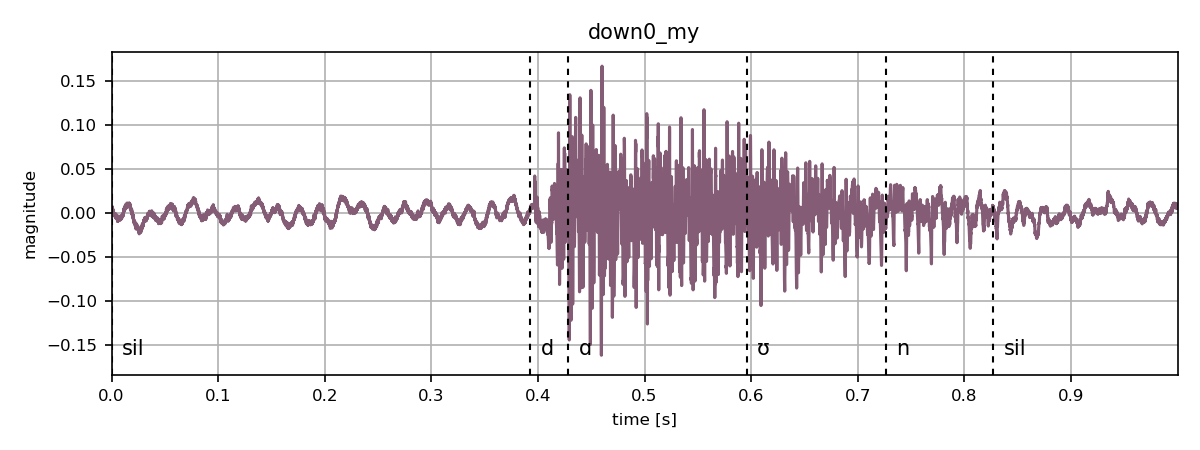
\includegraphics[width=0.65\textwidth]{./3_theory/figs/a1_raw/raw_down0_my}
    \subfigure[left]{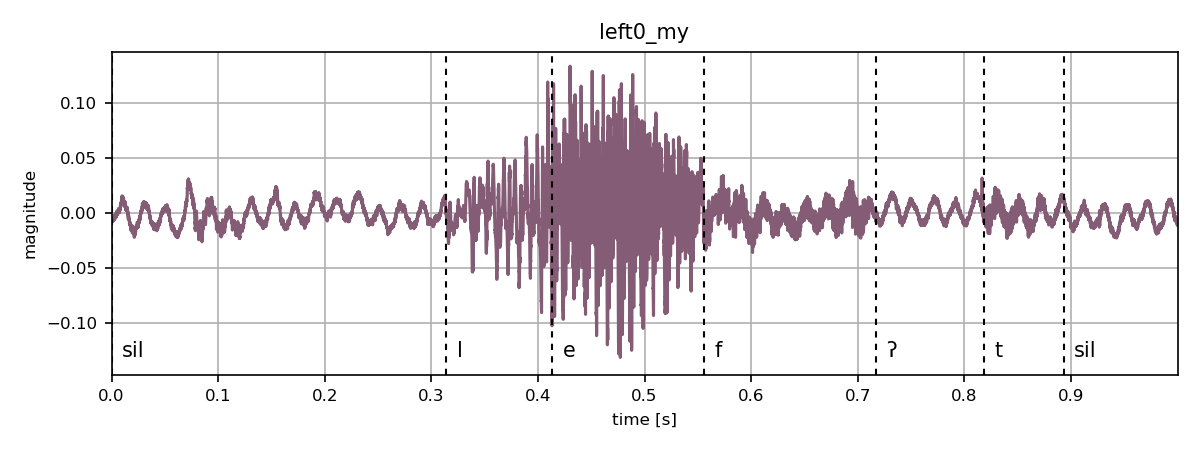
\includegraphics[width=0.45\textwidth]{./3_theory/figs/a1_raw/raw_left0_my}}
    \subfigure[right]{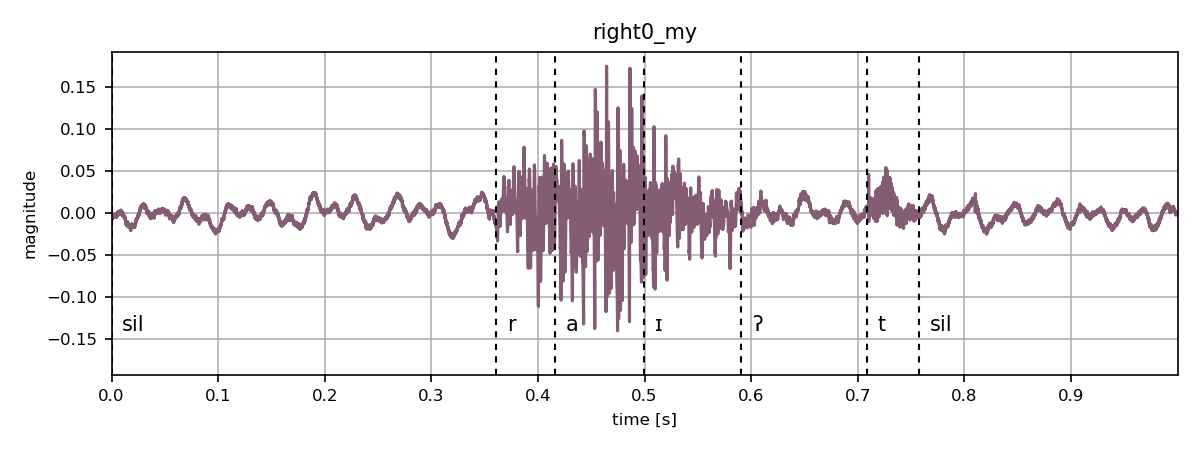
\includegraphics[width=0.45\textwidth]{./3_theory/figs/a1_raw/raw_right0_my}}
    \subfigure[up]{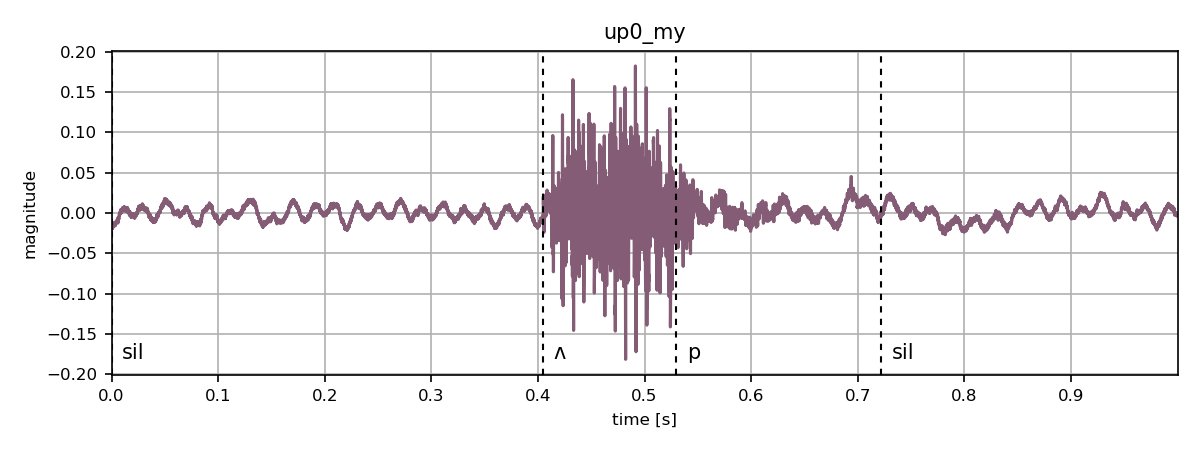
\includegraphics[width=0.45\textwidth]{./3_theory/figs/a1_raw/raw_up0_my}}
    \subfigure[down]{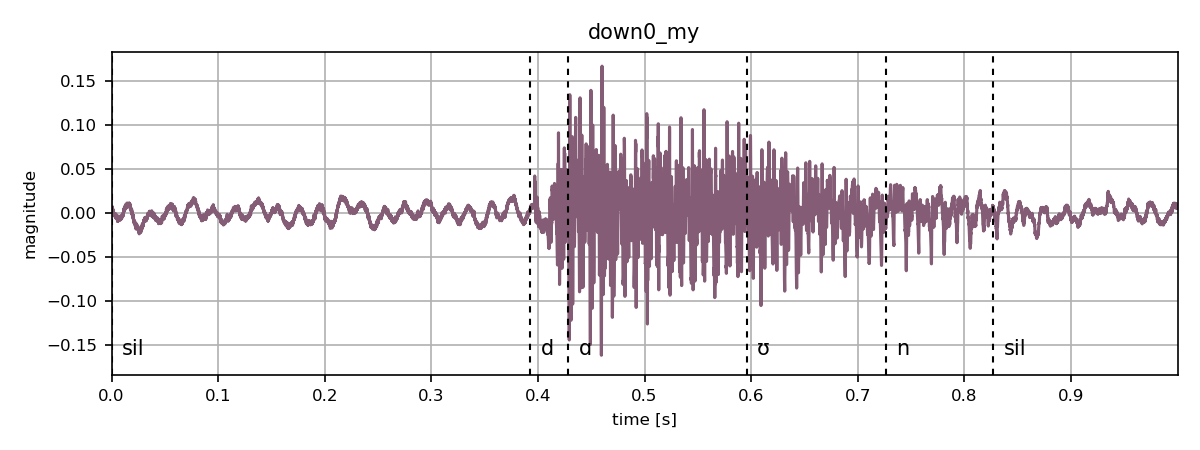
\includegraphics[width=0.45\textwidth]{./3_theory/figs/a1_raw/raw_down0_my}}
    \subfigure[go]{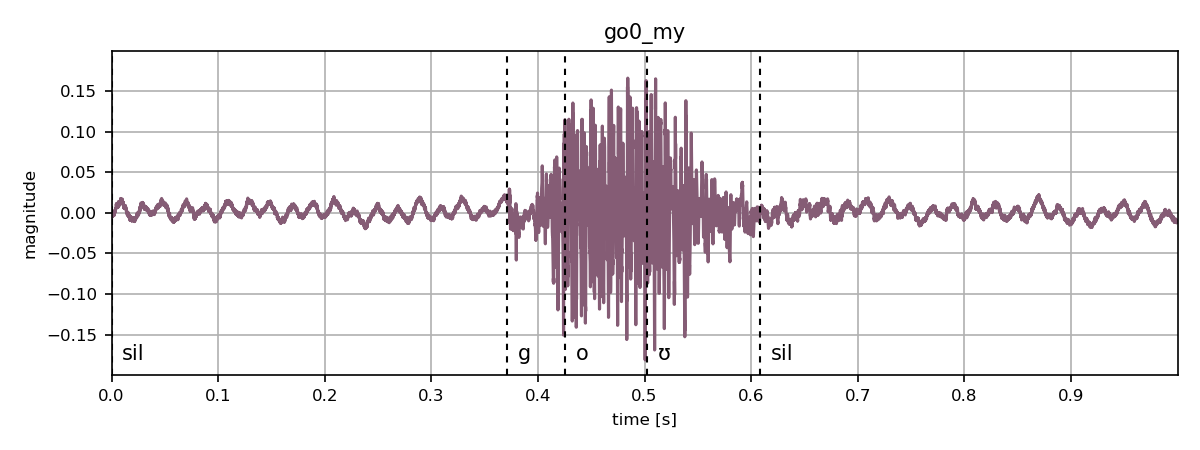
\includegraphics[width=0.45\textwidth]{./3_theory/figs/a1_raw/raw_go0_my}}
  \caption{Raw audio waveform files, recorded and annotated by the author with $f_s=16kHz$ and a simple consumer lavalier microphone.}
  \label{fig:raw_audio_my}
\end{figure}
\FloatBarrier
\noindent
From the raw audio files with annotations, one can observe that and estimate how long a speech command may take in terms of time and see that usually a whole second is too much for a single speech command.
Of course one can pronounce words longer or shorter, but usually in commanding something it is preferred to speak short well pronounced.
If a time interval of 500ms is used to capture a speech command (this time interval is used in the feature extraction for the machine learning), it might happen that not every phonetic letter of the words are captured. For instance this might happen often for words with glottal stops before consonants, as the phoneme \enquote{t} in \enquote{left} or \enquote{right}.
So the input features may only have information of the first phonetics, e.g. \enquote{lef} or \enquote{righ}, but since Key Word Spotting is restricted in its vocabulary, it should be no problem in distinguishing these two words when using a time interval of 500ms.

Another important point is to detect where the onset of the speech command is located on the time axis. It is easy to see in \rfig{raw_audio_my} where the words are starting, but usually not all recordings are as clean as those.
There might be a huge noise level or background noise and it is difficult to find the right onset position for the 500ms time interval with the 1s recordings.
For this Question to answer, it is postponed to the next sections on feature extraction.
At last it should be noted, that the value range in the y-axis of audio recordings strongly depends on the microphone, amplifiers and post processing.
It is naturally that all recording must be normalized to a specific value range, usually $[-1, 1]$.
\subsection{Spectral Features}
Spectral Features, such as a spectogram, are the most intuitive form to represent audio data. 
They show which frequencies are active at a time instance sampled at the hop time, the time on which the analytic window is shifted forward.

A spectogram with linear representation is shown in \rfig{spec-lin}.

\begin{figure}[!ht]
  \centering
    \subfigure[left]{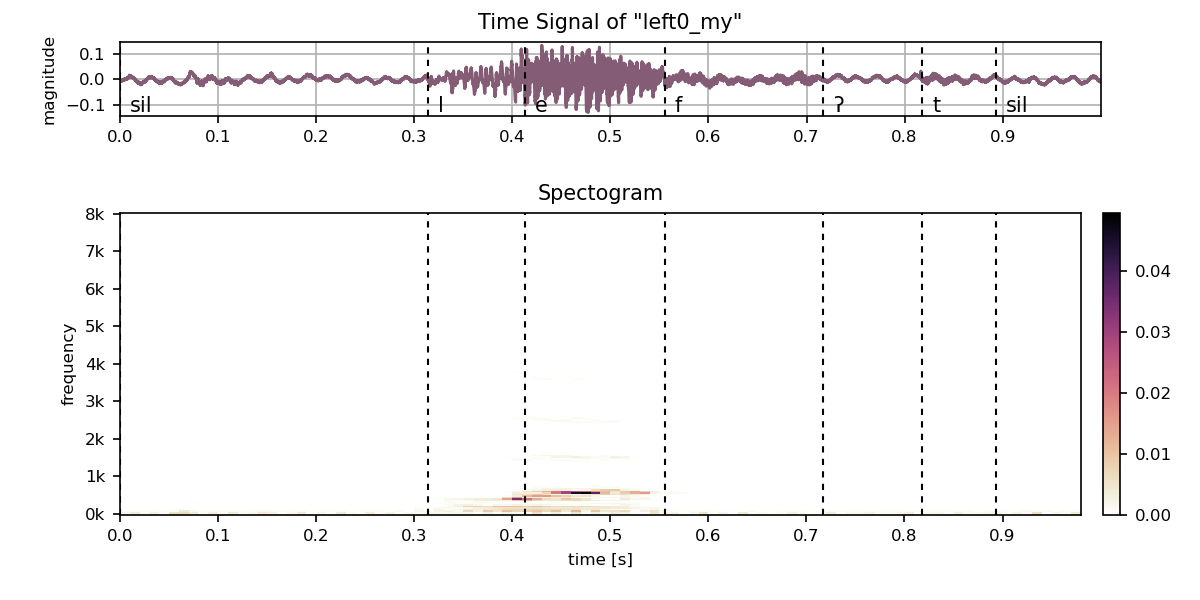
\includegraphics[width=0.45\textwidth]{./3_theory/figs/a2_spectogram/spec-lin_left0_my}}
    \subfigure[right]{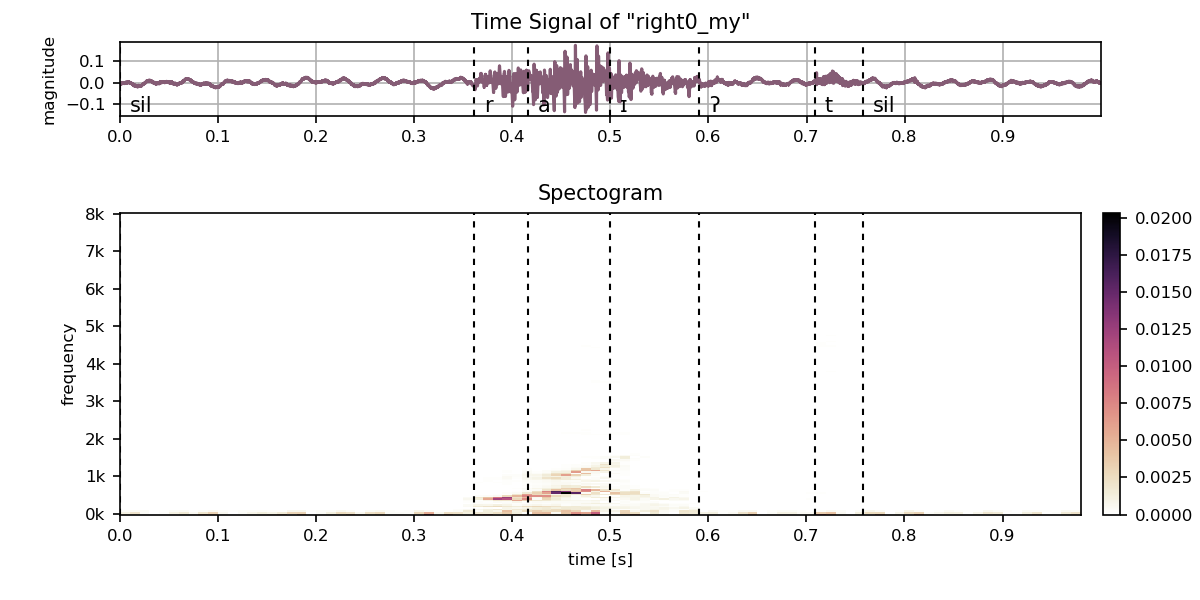
\includegraphics[width=0.45\textwidth]{./3_theory/figs/a2_spectogram/spec-lin_right0_my}}
    \subfigure[up]{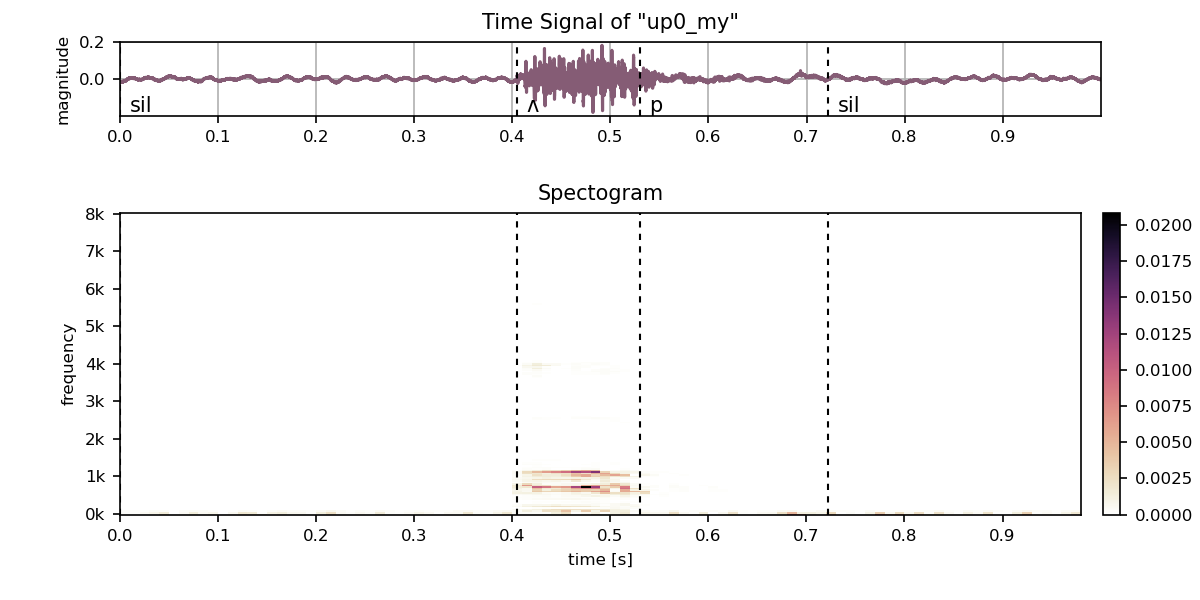
\includegraphics[width=0.45\textwidth]{./3_theory/figs/a2_spectogram/spec-lin_up0_my}}
    \subfigure[down]{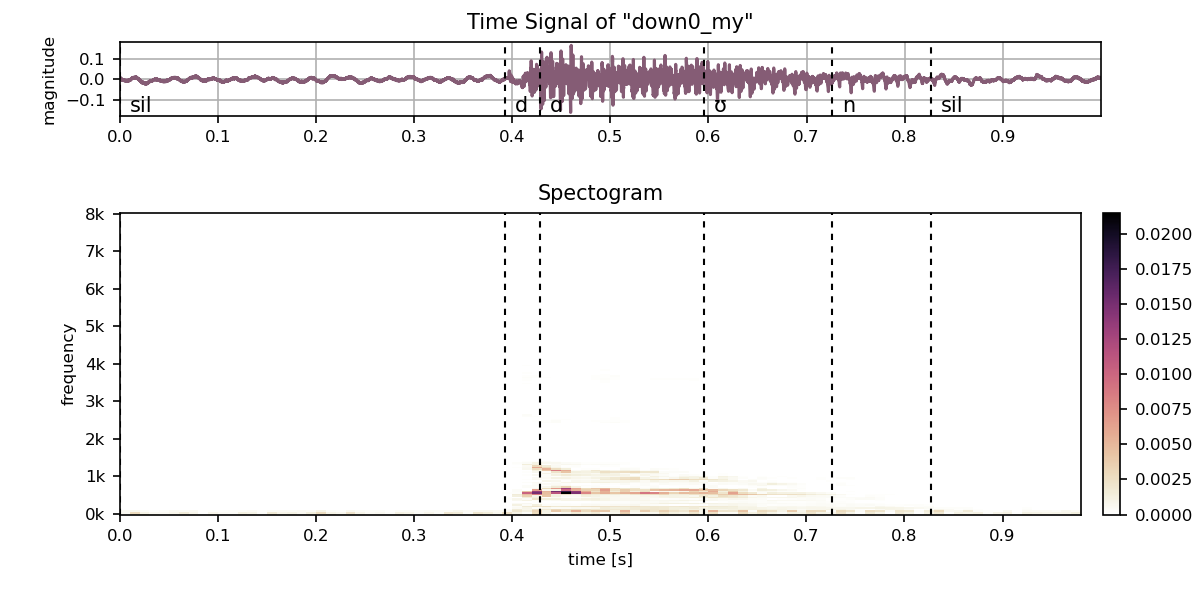
\includegraphics[width=0.45\textwidth]{./3_theory/figs/a2_spectogram/spec-lin_down0_my}}
    \subfigure[go]{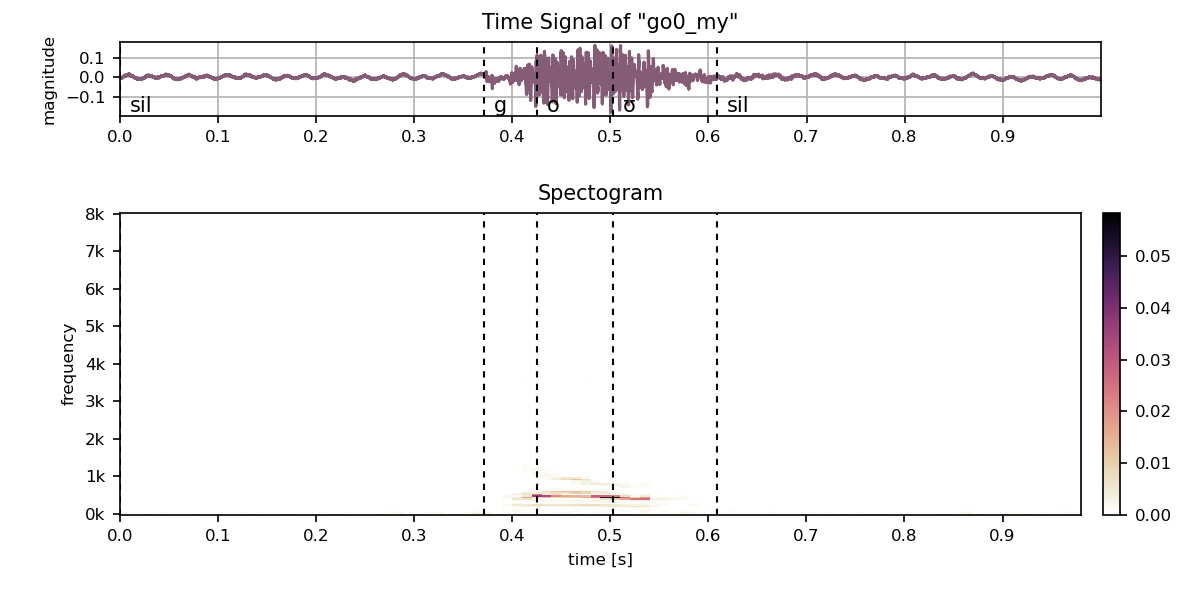
\includegraphics[width=0.45\textwidth]{./3_theory/figs/a2_spectogram/spec-lin_go0_my}}
  \caption{Spectogram linear scaled.}
  \label{fig:spec-lin}
\end{figure}
\FloatBarrier
\noindent

One can see here, that most of the energy of the signal is in the lower frquency regions under 1kHz.
It is more interesting to go into the log scale, shown in \rfig{spec-log}

\begin{figure}[!ht]
  \centering
    \subfigure[left]{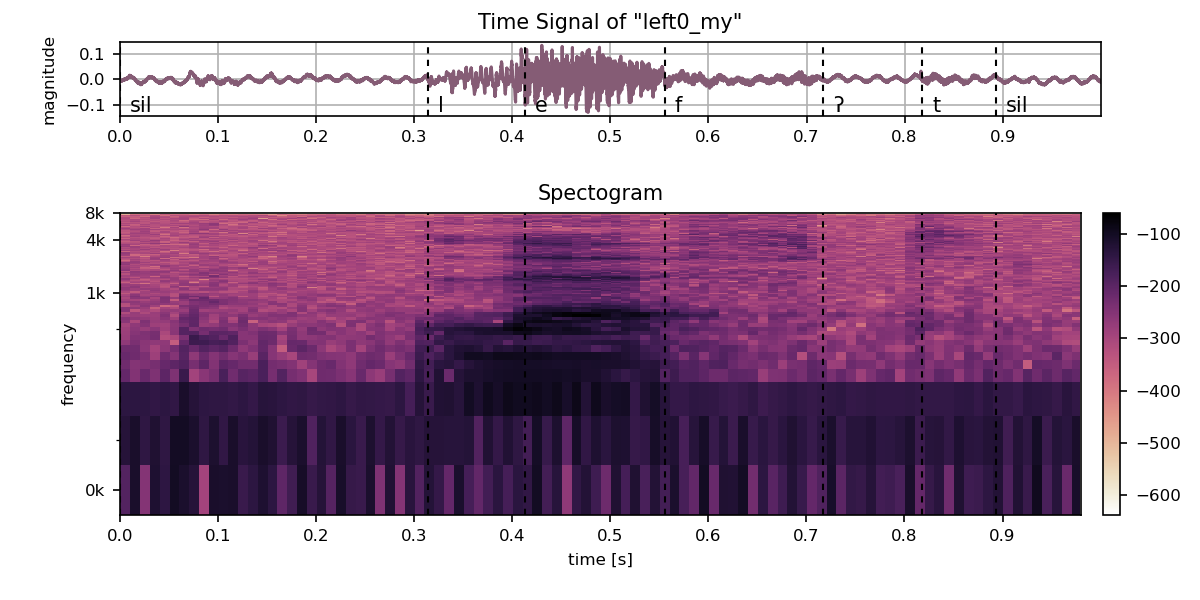
\includegraphics[width=0.45\textwidth]{./3_theory/figs/a2_spectogram/spec-log_left0_my}}
    \subfigure[right]{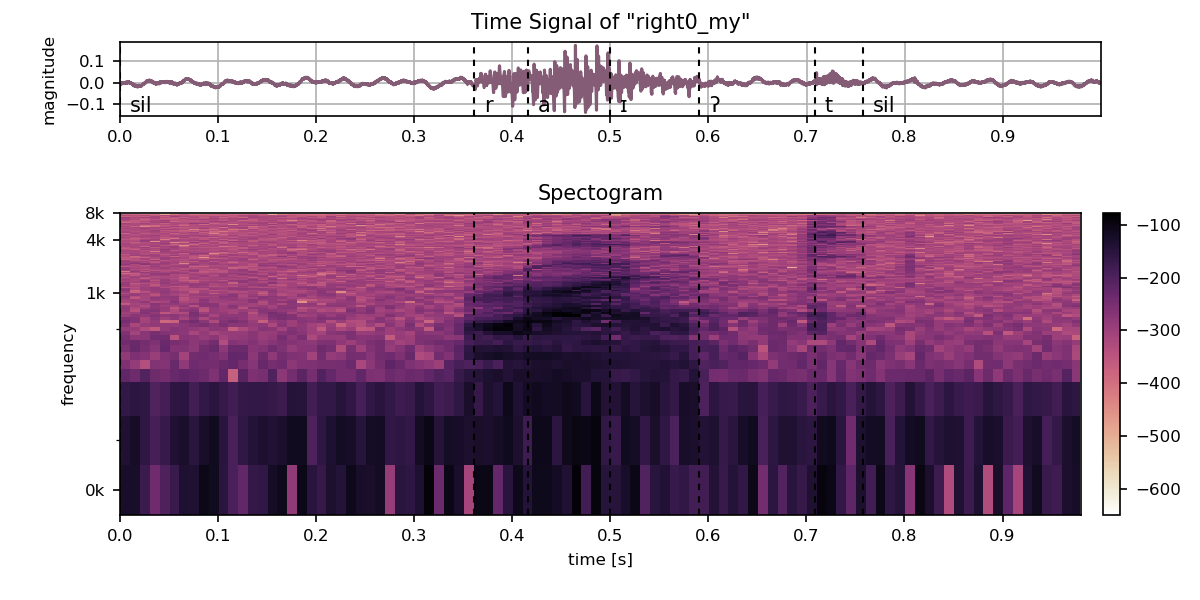
\includegraphics[width=0.45\textwidth]{./3_theory/figs/a2_spectogram/spec-log_right0_my}}
    \subfigure[up]{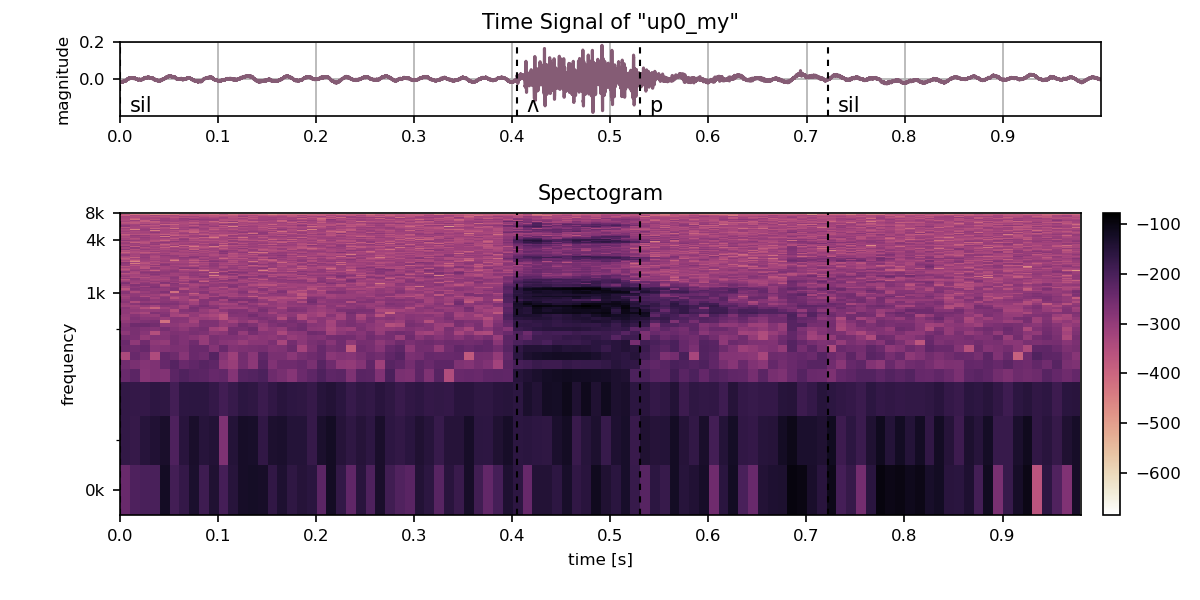
\includegraphics[width=0.45\textwidth]{./3_theory/figs/a2_spectogram/spec-log_up0_my}}
    \subfigure[down]{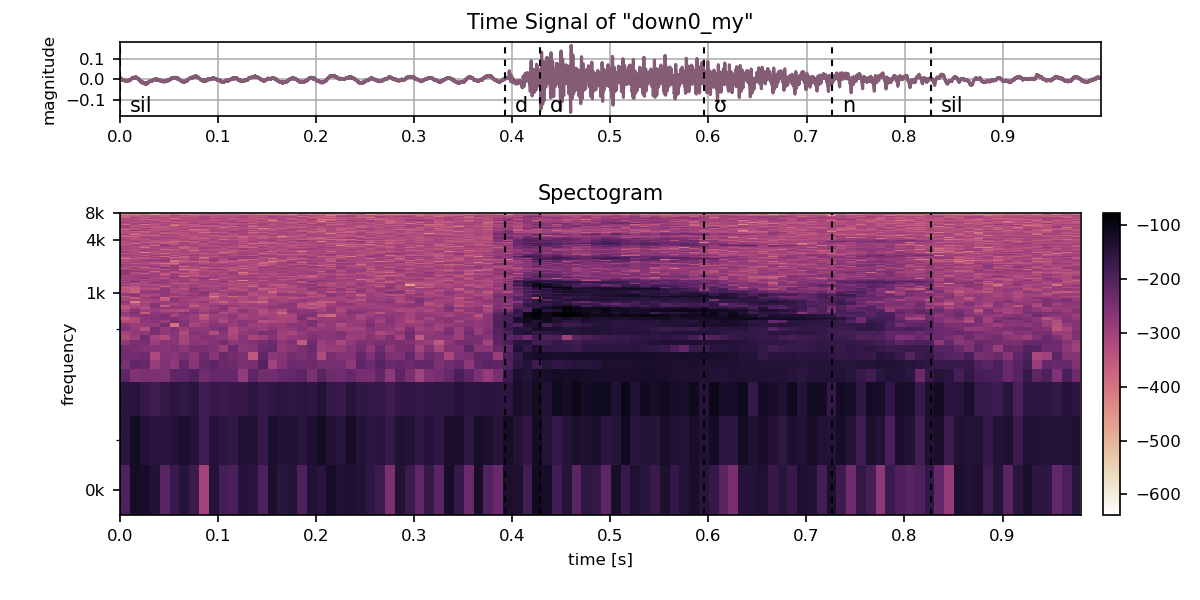
\includegraphics[width=0.45\textwidth]{./3_theory/figs/a2_spectogram/spec-log_down0_my}}
    \subfigure[go]{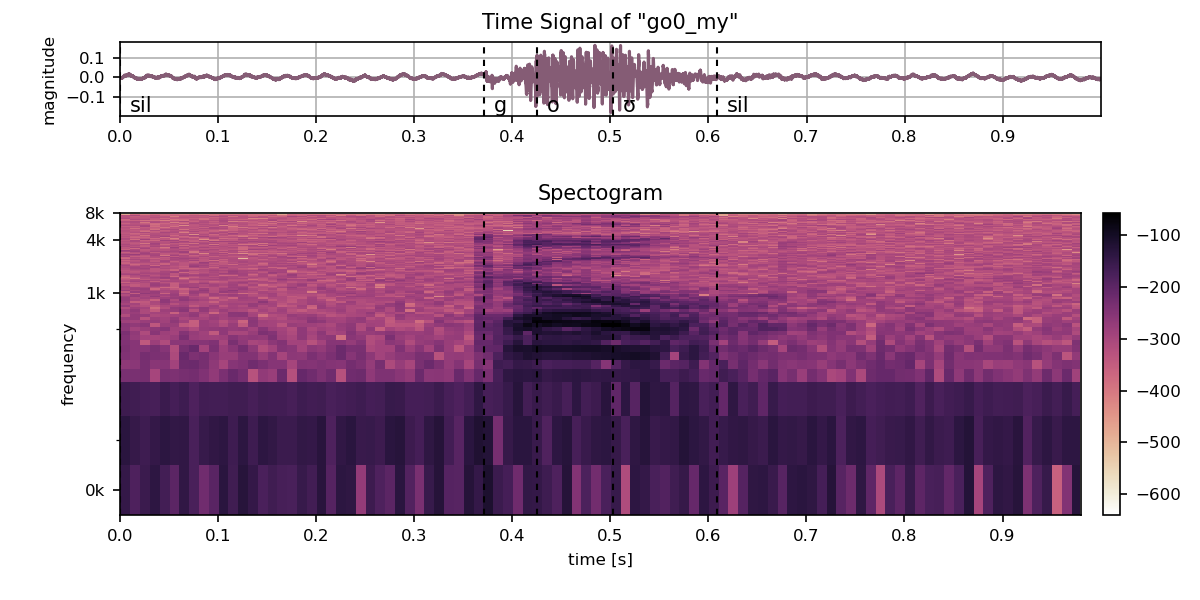
\includegraphics[width=0.45\textwidth]{./3_theory/figs/a2_spectogram/spec-log_go0_my}}
  \caption{Spectogram logarithmic scaled.}
  \label{fig:spec-log}
\end{figure}
\FloatBarrier
\noindent
% --
% mfcc

\subsection{Mel Frequency Coefficients}\label{sec:t_mfcc}
Most commonly the Mel Frequency Cepstral Coefficients (MFCC) are used as input features for Neural Network classifications tasks of audio data.
It is described why they are good features and how they can be visualized to understand them better.

\subsubsection{About Mel Frequency Cepstral Coefficients}
To comprehend the success of the wide use of MFCCs features in Neural Networks and other machine learning applications, it is necessary to understand its processing scheme, which is roughly as following: 
Raw input data is transformed into the frequency domain with an STFT, the power spectrum of this STFT is then segmented into a filter bank with equidistant mel frequencies, then logarithmic scaling is done and as last step a decorrelation with the DCT transform.
Which seem quite complicated at the beginning, is in fact nothing else but some reasonable steps of data compression. 
It is also possible to input a spectrum to the Neural Network, but the amount of input data is just too much.
That is why frequencies are put in certain bands through a filter bank and further decorrelated with a method like the DCT.

\subsubsection{Processing Pipeline and Background}
The frequency spectrum is spitted into filter bands, done by triangular window functions.
These window functions must have a fixed length on the mel space (equidistant mel bands), that results in different spacings of
the frequency space. The mel and frequency window functions are shown in \rfig{filter_bands}.
\begin{figure}[!ht]
  \centering
  \subfigure[mel space]{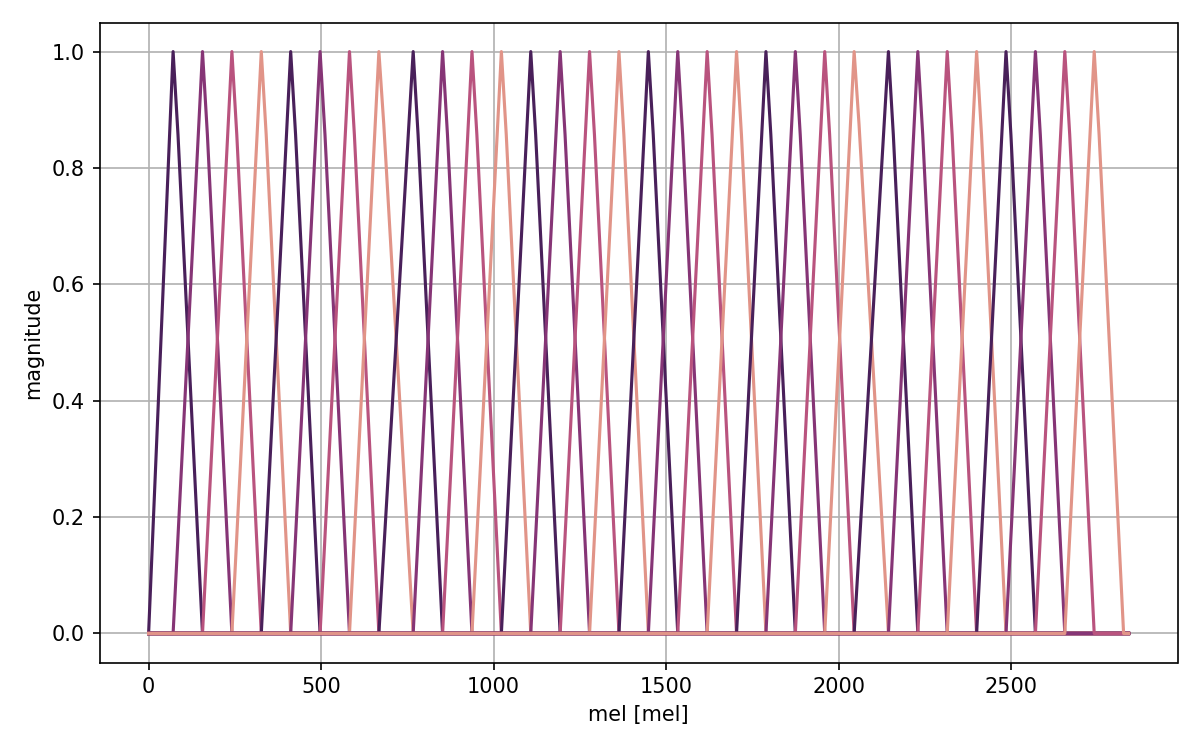
\includegraphics[width=0.40\textwidth]{./3_theory/figs/a3_mfcc/weights_mel}}
  \quad
  \subfigure[frequency space]{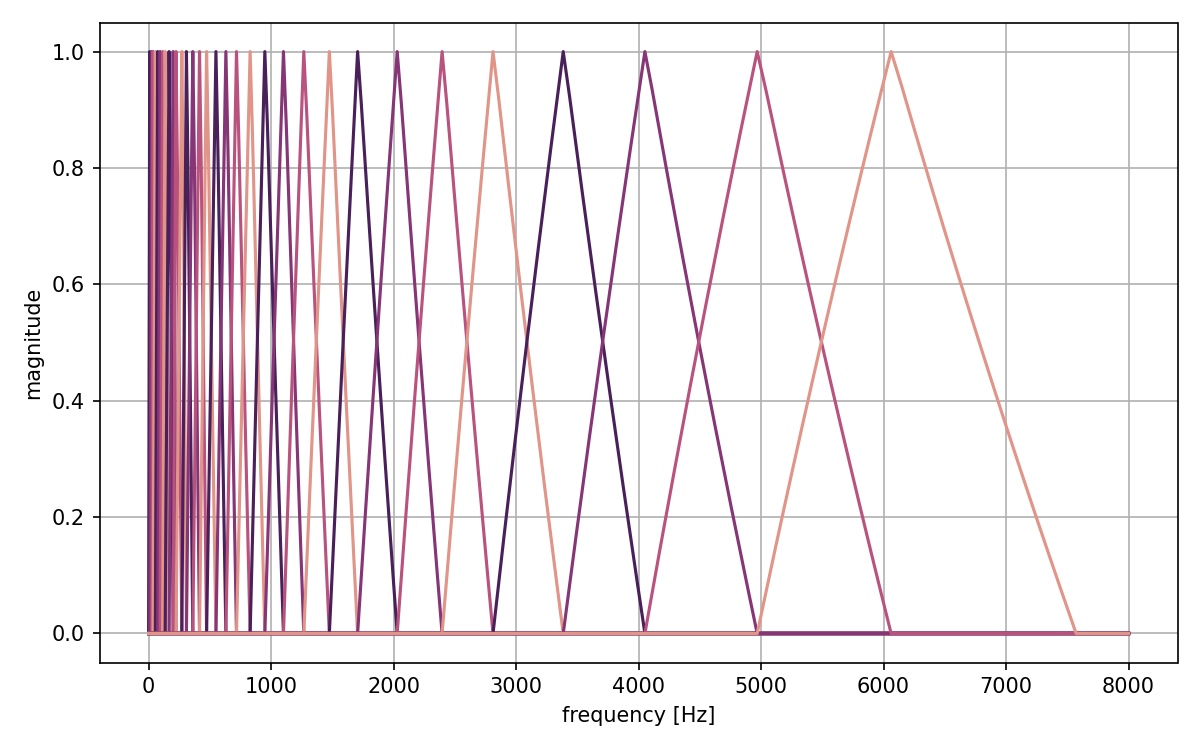
\includegraphics[width=0.40\textwidth]{./3_theory/figs/a3_mfcc/weights_f}}
  \caption{Equidistant mel filter bands with a total number of 32 bands.}
  \label{fig:filter_bands}
\end{figure}
\FloatBarrier
\noindent

The DCT is similar to the Fourier Transform and projects the input signal to a set of basis functions. 
These Basis functions are illustrated in \rfig{dct}
\begin{figure}[!ht]
  \centering
  \subfigure[DCT with continuous color scheme]{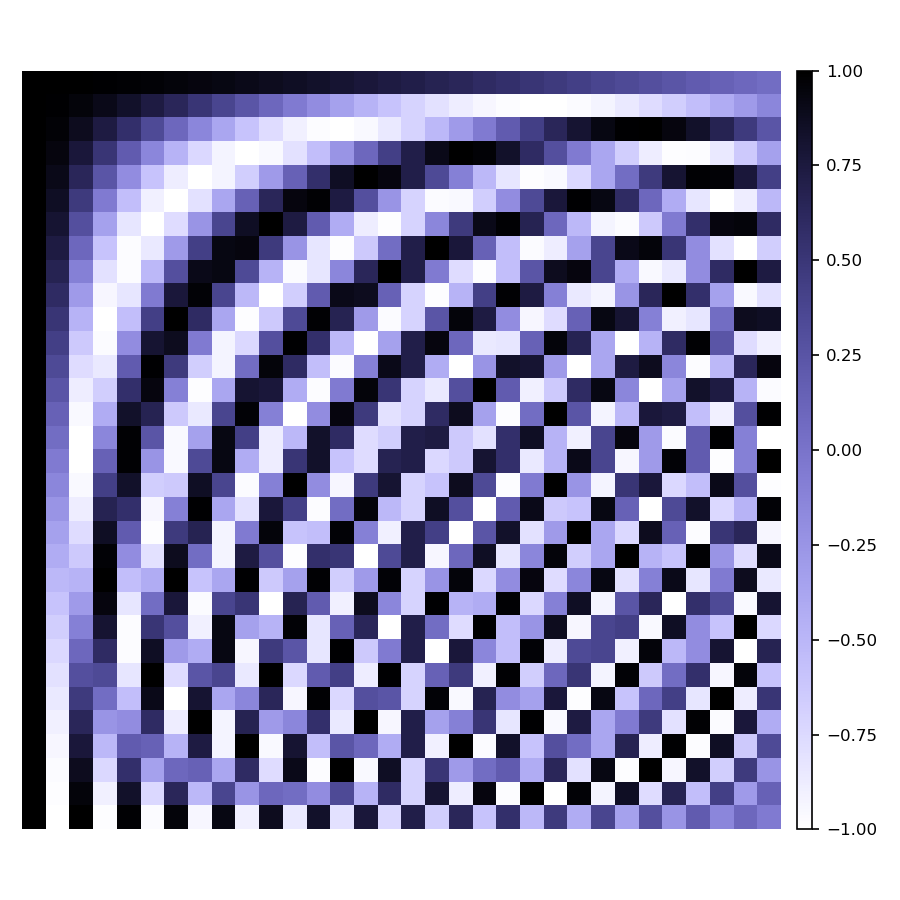
\includegraphics[width=0.40\textwidth]{./3_theory/figs/a3_mfcc/dct}}
  \quad
  \subfigure[DCT with diverging color scheme]{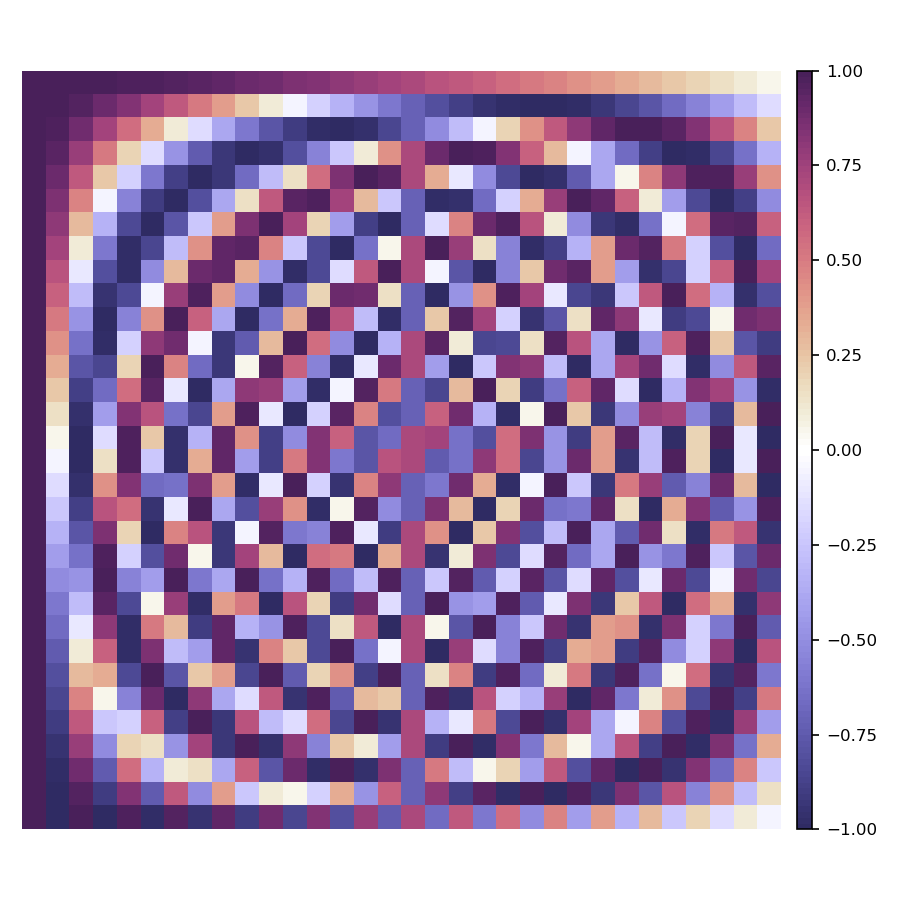
\includegraphics[width=0.40\textwidth]{./3_theory/figs/a3_mfcc/dct-div}}
  \caption{DCT matrix with 32 basis functions illustrated with a continuous and a diverging color scheme.}
  \label{fig:dct}
\end{figure}
\FloatBarrier
\noindent


\subsubsection{MFCC Feature Usage and Enhancement}
After the MFCCs are computed, they can be used as input features for Neural Networks. 
The important Question here is whether an feature enhancement can be done and if all those computed features are necessarily and meaningful for the training and evaluation success of Neural Networks. Usually not all MFCC coefficients are used as inputs, this is merely done to reduce the computational cost in case the accuracy does not suffer from it.
A good application is to compute 32 MFCC features (with 32 equidistant Mel filter bands) and use only the first 12 of them as inputs.
Further it is also possible to compute derivatives (in the time domain) of MFCC features, denoted as Deltas. 
Those derivatives are simple computed as frame difference of the MFCCs.
A second derivative of MFCC features, known as Double Deltas, are then the frame differences of the Deltas.
At last an energy feature can be computed from each of the MFCCs, Deltas and Double Deltas, each by its own and added to the feature vectors.
Those feature vectors can then be simply stacked at top of each other and used as feature inputs.
In this thesis the feature vectors are stacked as following:
\begin{enumerate}
    \item 12 MFCCs
    \item 1 Energy feature of the 12 MFCCs
    \item 12 Deltas
    \item 1 Energy feature of the 12 Deltas
    \item 12 Double Deltas
    \item 1 Energy feature of the 12 Double Deltas
\end{enumerate}
Which sums up to a 39-dimensional feature vector.

\subsubsection{Visualisation of MFCC features}
A good visualisation of MFCC features is the best way to understand them.
With this thought in mind, much time was spent to create a fitting visual representation of the MFCC features, but this was not an easy task.
MFCCs are not well intended for visualisations, since their individual coefficients value space, can be strongly different from each other.
For example, the first coefficient equals a summation of all filter bands and is therefore some kind of energy measure over all bands, while the other coefficients are weighted sum combinations of the filter bands.
This alone yields in totally different value spaces and value spaces should not differ that much, when features should be represented with colors.
Further it is to mention, that most of the signal energy will be in the lower frequency bands, which also impacts the value space of the individual coefficients a lot.
To show this difference in value space in a negative example in practise, the MFCCs of the self-recorded speech command waveform \enquote{left0.wav} is shown in \rfig{left0_mfcc_only}.

\begin{figure}[!ht]
  \centering
    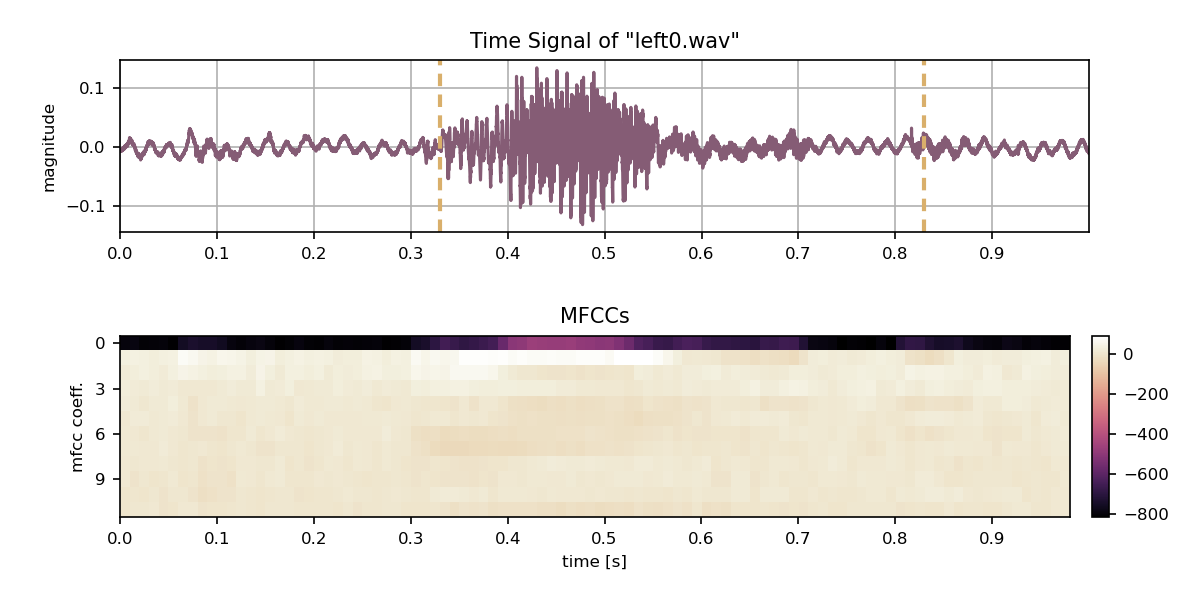
\includegraphics[width=0.75\textwidth]{./3_theory/figs/a3_mfcc/left0_mfcc_only.png}
  \caption{Bad visualisation of the 12 MFCCs features extracted from \enquote{left0.wav}.}
  \label{fig:left0_mfcc_only}
\end{figure}
\FloatBarrier
\noindent
Not much structure of the MFCCs can be seen here, due to the vast value difference of the first coefficient. At least the first coefficient shows, where the center of signal energy is placed on the time scale, but other than that, this visualisation is worthless.
Another very bad visualisation is shown by computing the 39 MFCC feature vectors (with Deltas, Double Deltas and Energies) in \rfig{left0_no_order}.

\begin{figure}[!ht]
  \centering
    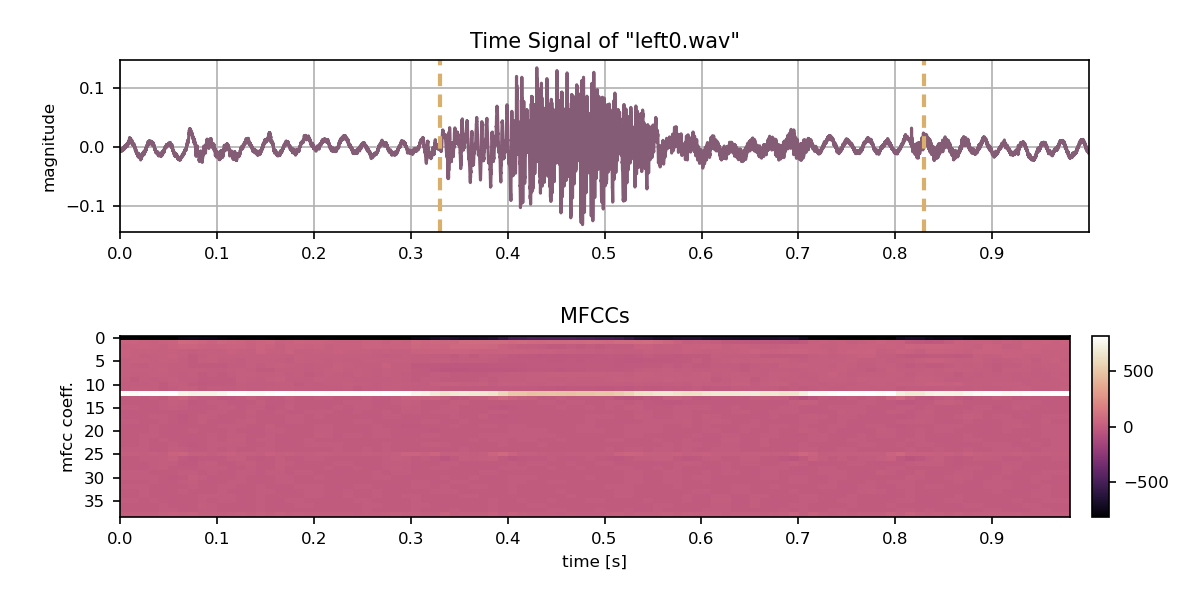
\includegraphics[width=0.75\textwidth]{./3_theory/figs/a3_mfcc/left0_no_order_norm0.png}
  \caption{Very bad visualisation of 39 MFCC features extracted from \enquote{left0.wav}.}
  \label{fig:left0_no_order}
\end{figure}
\FloatBarrier
\noindent
There appears an even greater gap of different value spaces and even less is seen.
One very easy solution is to show the features in different value groups. For instance the first coefficient and its deltas is in one group, the other coefficients in another and the deltas and energies are separated as well in own groups. Now we actually can see some structure in the visualisations, shown in \rfig{left0_order}.

\begin{figure}[!ht]
  \centering
    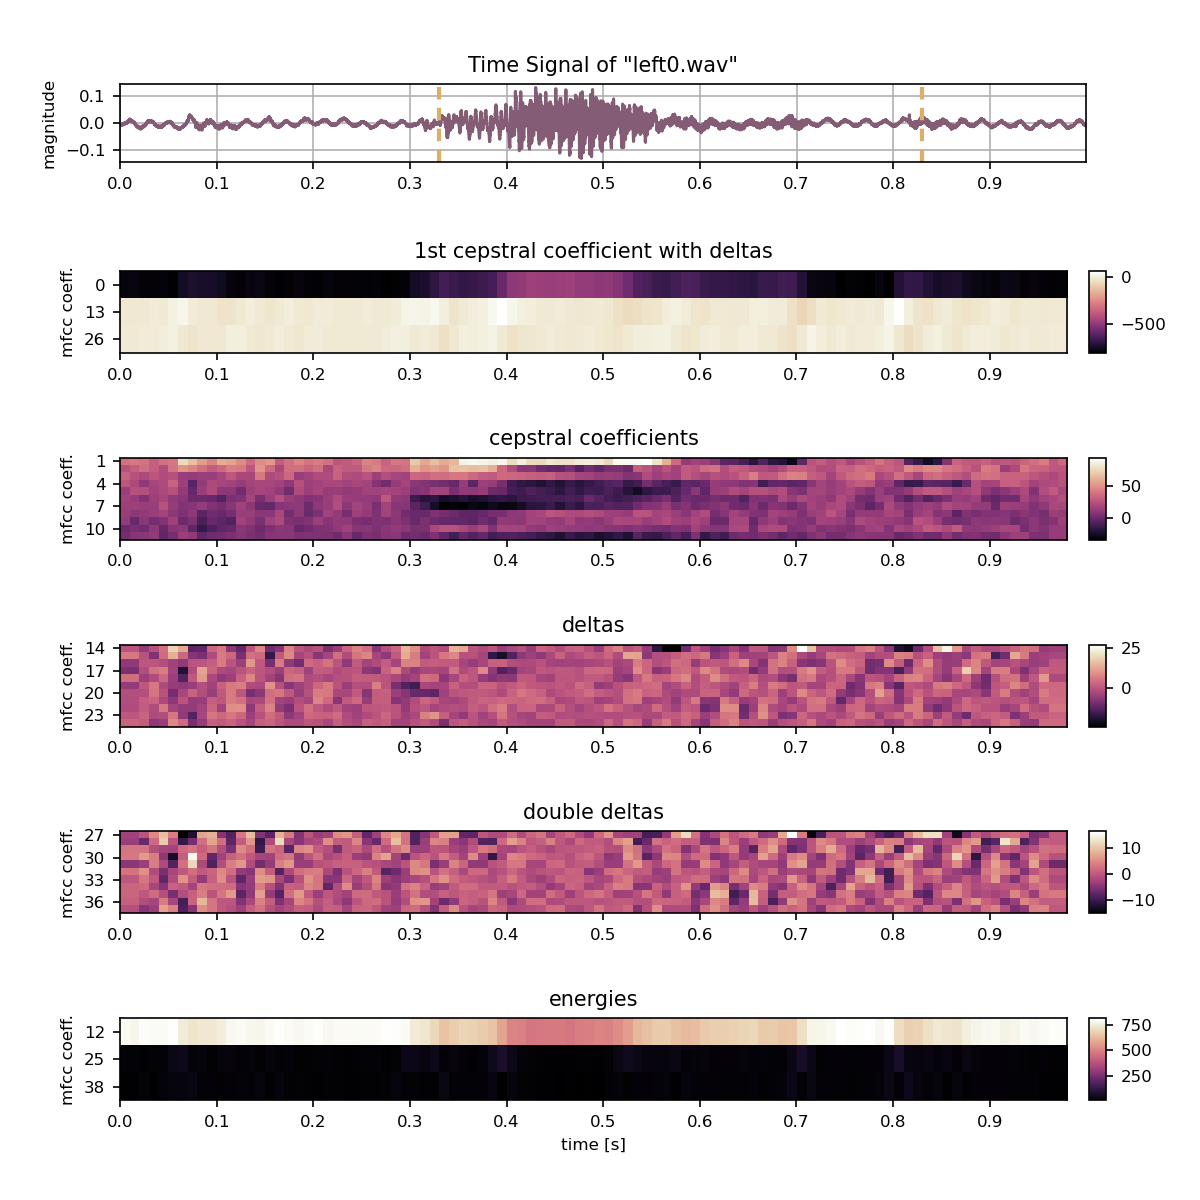
\includegraphics[width=0.75\textwidth]{./3_theory/figs/a3_mfcc/left0_norm0.png}
  \caption{Good visualisation of 39 MFCC features extracted from \enquote{left0.wav} with own value groupings.}
  \label{fig:left0_order}
\end{figure}
\FloatBarrier
\noindent
Another way to improve the visualisation is to normalize the feature vectors over their each own frame dimension with the infinity norm. This will yield a value space of $[0, 1]$ for each feature vector. With this, the visualisation of the 39 MFCC of \enquote{left0.wav} is shown in \rfig{left0_order},

\begin{figure}[!ht]
  \centering
    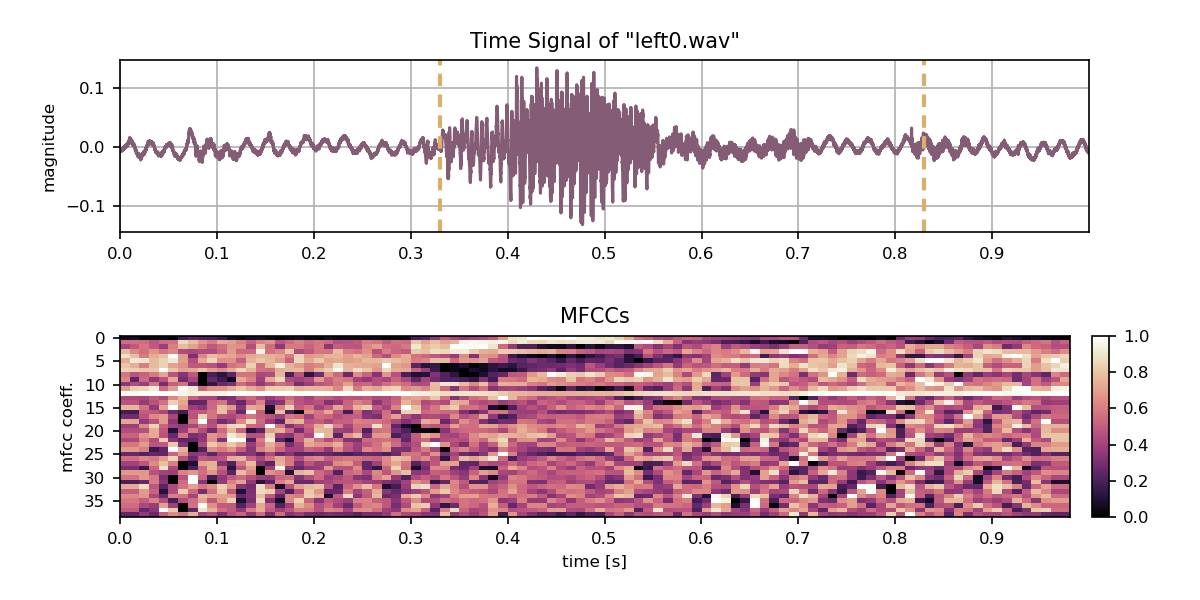
\includegraphics[width=0.75\textwidth]{./3_theory/figs/a3_mfcc/left0_no_order_norm1.png}
  \caption{Normalisation of 39 MFCC features extracted from \enquote{left0.wav}.}
  \label{fig:left0_no_order_norm1}
\end{figure}
\FloatBarrier
\noindent
or in an even better one shown in \rfig{left0_order_norm1}.

\begin{figure}[!ht]
  \centering
    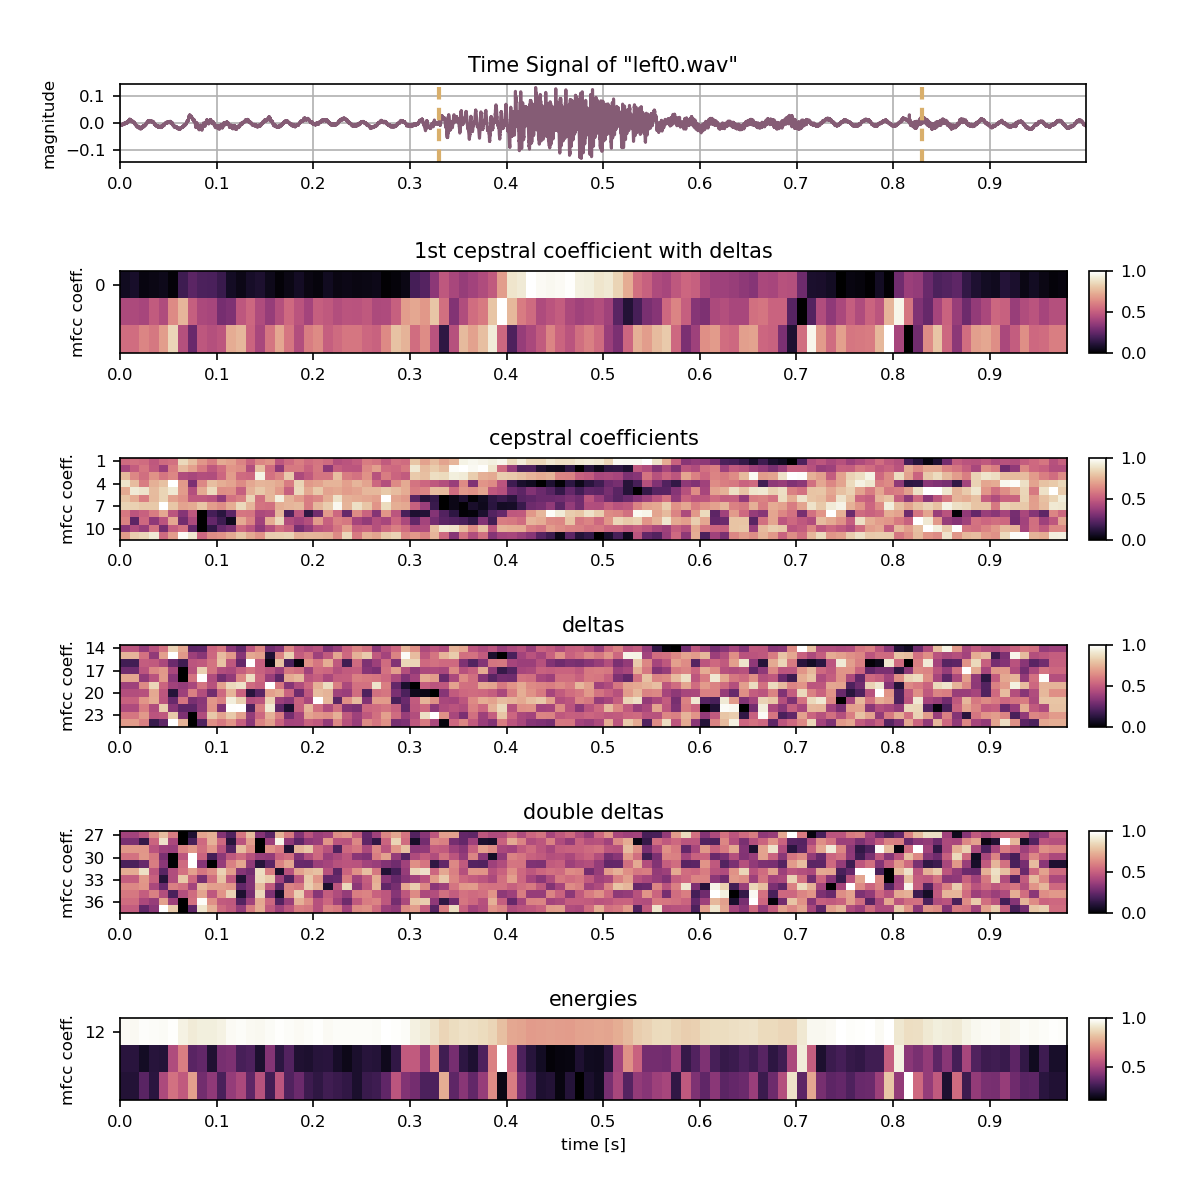
\includegraphics[width=0.75\textwidth]{./3_theory/figs/a3_mfcc/left0_order_norm1.png}
  \caption{Normalisation of 39 MFCC features extracted from \enquote{left0.wav} with groups.}
  \label{fig:left0_order_norm1}
\end{figure}
\FloatBarrier
\noindent
As conclusion, the normalisation in the frame space is an interesting aspect to improve the visualisation of the MFCC features, 
specifically for the cepstral coefficients and the energy features (not the deltas).
Exactly this nice representation was motivating to explore normalisation of feature for Neural Network inputs.
However this is a very crucial thing to do. A normalisation relatives important structures within the feature space and it cannot really be answered if this is a good thing or not.
One more research question arises here: Is it possible to use normalisation for the features as inputs to Neural Networks and what are the results to the accuracy and training of the models.


% ml
\section{Machine Learning Theory}
theory...
\subsection{Neural Network Architectures}\label{sec:nn_arch}
All Neural Network Architectures evaluated within this thesis are presented here.
%There will be a general classification between Neural Network Architectures by Convolutional Neural Networks, Adversarial Neural Networks ...
In general the architectures can be differentiated between:
\begin{enumerate}
	\item Convolutional Neural Networks
	\item Adversarial Neural Networks
	\item Wavenets
\end{enumerate}
The term Convolutional Neural Networks here consists of all architectures consisting of at least one convolutional layer and the intention to simply classify each speech commands from each other. 
Therefore the output of a Convolutional net is of size of the amount of speech commands and usually has some kind of probability distribution or energy equivalence.

With Adversarial Neural Networks all architectures are meant, with at least two separate Neural Network Architectures, e.g. a Discriminator and a Generator Network and the intention to outperform the other Network in a task where both play a game against each other.
The word game here, is used in the sense of Game Theory, where the goal is to find an equilibrium state where both players are equally satisfied with the state.

An overview of all models is shown in \rtab{nn_arch_overview} with abbreviations in \rtab{nn_arch_abbreviation}.
\begin{table}[ht!]
\begin{center}
\caption{Network Architectures Abbreviations}
\begin{tabular}{ M{2.5cm}  M{10cm} }
\toprule
\textbf{Abbreviations} & \textbf{Meaning}\\
\midrule
c[0-9] & convolutional layer with layer number\\
f[0-9] & feed forward fully connected layer with layer number\\
m[0-9] & max pooling layer layer with layer number\\
ch & input channel number for mfccs it is usually 1\\
fs & frame size (usually 50 -> 50ms)\\
ms & feature size (mfcc), depends on feature selection\\
cf & output number of last flattened convolutional layer\\
cl & number of class labels\\
\bottomrule
\label{tab:nn_arch_abbreviation}
\end{tabular}
\end{center}
\end{table}
\FloatBarrier
\noindent
\begin{table}[ht!]
\begin{center}
\caption{Network Architectures Overview with reference names}
\begin{tabular}{ M{2.5cm}  M{2.1cm}  M{2.1cm} M{2.1cm} M{2.5cm}}
\toprule
%\multicolumn{4}{c}{\textbf{Feature Groups}} & \multicolumn{2}{c}{\textbf{Accuracy}} \\
\textbf{Reference name} & \textbf{Feature maps} & \textbf{Kernel sizes} & \textbf{Strides} & \textbf{Feed Forward} \\
\midrule
conv-trad & c1: (ch, 64) c2: (64, 64) & c1: (4, 20) mp: (2, 4) c2: (2, 4) & c1: (1, 1) mp: (2, 4) c2: (1, 1) & f1: (cf, 32) \quad f2: (32, 128) f3: (128, cl)\\
\midrule
conv-fstride & c1: (ch, 54) & c1: (8, fs) & c1: (4, 1) & f1: (cf, 32) \quad f2: (32, 128) \quad f3: (128, 128) \quad f4: (128, cl)\\
\midrule
conv-encoder-fc1 & c1: (ch, 48) \quad c2: (48, 8) & c1: (ms, 20) \quad c2: (1, 5) & c1: (1, 1) \quad c2: (1, 1) & f1: (cf, cl)\\
\midrule
conv-encoder-fc3 & c1: (ch, 48) \quad c2: (48, 8) & c1: (ms, 20) \quad c2: (1, 5) & c1: (1, 1) \quad c2: (1, 1) & f1: (cf, 64) \quad f2: (64, 32) \quad f3: (32, l)\\
\bottomrule
\label{tab:nn_arch_overview}
\end{tabular}
\end{center}
\end{table}
\FloatBarrier
\noindent


\subsection{Adversarial Training Theory}\label{sec:adv_theory}
Working with adversarial Neural Networks is quite interesting, as two separate Networks are challenge themselves against each other to improve their performance.
The paper from Goodfellow et. al. \cite{goodfellow2014} describes a game between two Neural Networks (players), where one player has the role of creating fakes and the other must determine if it is real or fake.
The Network who creates fakes is called Generator (G) and the other Network who has to decide about fake or not is called Discriminator (D).
The Generators goal is to create fakes that look like reals, so that D makes mistakes and classifies a fake as a real.
On the other hand the Discriminator must also constantly improving itself, so that fakes from G can be detected and sorted out from the reals.

This approach works remarkably well to create a generative network able to produce fakes that are astonishing similar to real ones.
In the mentioned paper, this was applied to images and not for audio data.
But if the audio waveform is presented as spectogram or mfcc with fixed frame size, it can be seen as an image, where one dimension is time and the other frequency.

So far a generative network does only produce fake images and a discriminative network can only output a one dimensional (probability) output, to decide if it is fake or not.

The idea now is not to use either of these networks, but to use transfer learning in the sense to reuse the convolutional layers both networks achieved during their game (training).
The weights of those convolutional layers are then transfered to another network with classification purpose on multiple labels.

\subsubsection{Questions that arise}
There are several questions that arise regarding Adversarial Training:
\begin{enumerate}[label={Q.\textgoth{A}.\arabic*)}, leftmargin=1.4cm]
  \item Does the Network Architecture of G and D have to be the same but transposed?
  \item Does the value space of in and outputs, for D and G respectively, have to be limited e.g. [0, 1] done by e.g. frame normalization, or sigmoid output?
  \item What loss function works well for training?
  \item How long should be trained?
  \item When transfering weights to another network, should the weights from G or D be transfered?
  \item Does the classification network has to adapt the parameters from the transfered weights?
  \item Whats the benefit of all this?
\end{enumerate}

To illustrate the idea an example is shown of the labels L5 (left, right, up, down, go).

The convolutional layer weights from the adversarial training of the individual labels, 
can be stacked together an used to initialize another network.
An example of this method is shown in \rfig{ml_adv_example}, where the initialization pattern changes to more elaborate structures and patterns to form good classification outputs. 
However the Basic Pattern from the adversarial training stays the same, which is a good sign, because then the network is accepting those trained weights and adapts them.

\begin{figure}[!ht]
  \centering
    \subfigure[c1 trained]{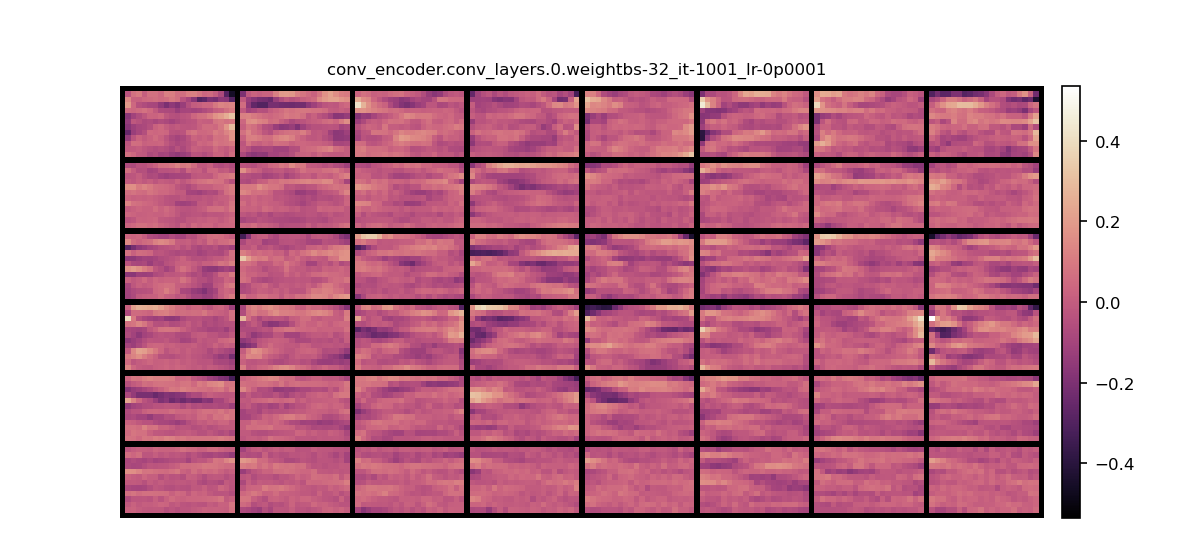
\includegraphics[width=0.45\textwidth]{./3_theory/figs/ml_adv_example_c0}}
    \subfigure[c1 init]{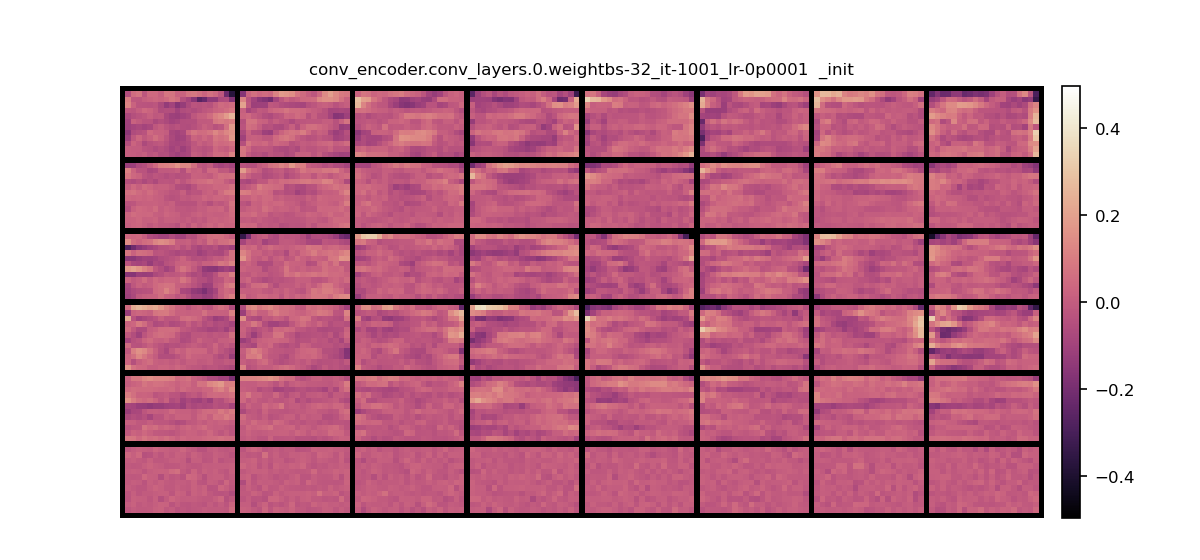
\includegraphics[width=0.45\textwidth]{./3_theory/figs/ml_adv_example_c0_init}}
    \subfigure[c2 trained]{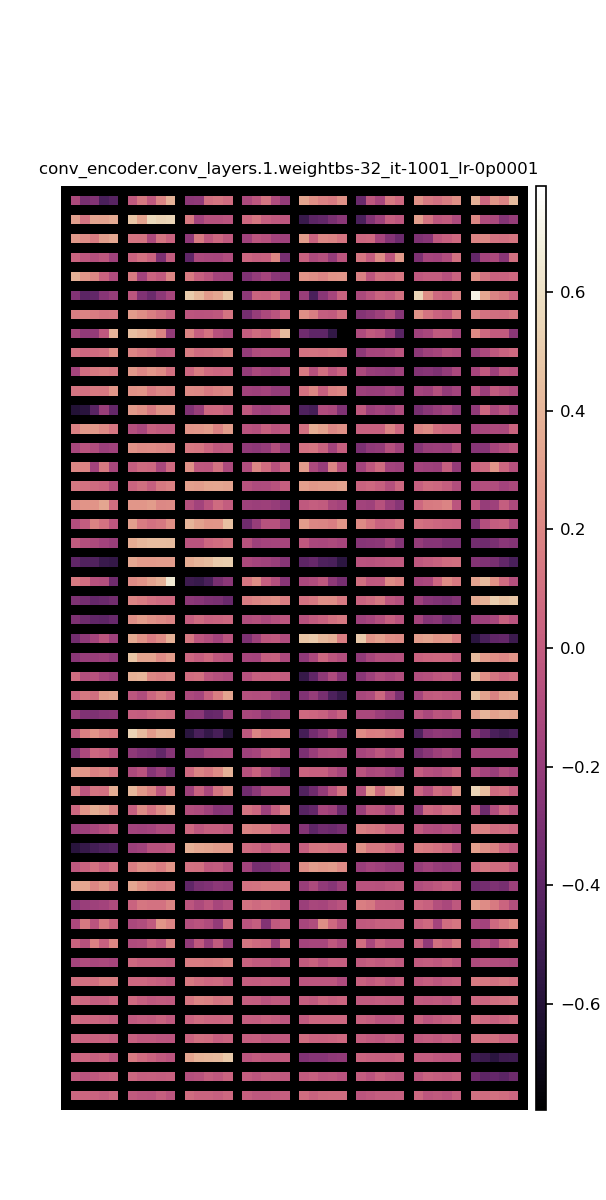
\includegraphics[height=0.45\textwidth]{./3_theory/figs/ml_adv_example_c1}}
    \quad
    \subfigure[c2 init]{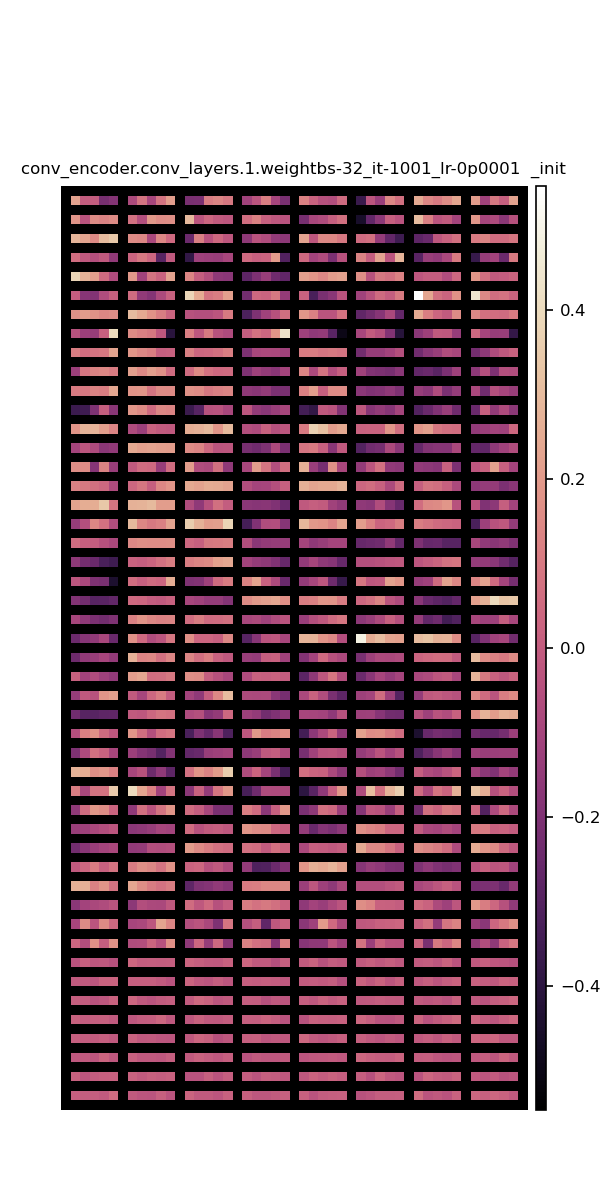
\includegraphics[height=0.45\textwidth]{./3_theory/figs/ml_adv_example_c1_init}}
  \caption{Adversarial Training Example: Convolutional layers pretrained with adversarial training on each label separately.}
  \label{fig:ml_adv_example}
\end{figure}
\FloatBarrier
\noindent

For this example in adversarial training, 8 feature maps of the first layer were used for each label, also they belong to the Generator Network G or decoder (dec). In Convolutional Networks, each previous layers feature map creates a new set of feature maps in the next layer.
An example of this label training is shown in \rfig{ml_adv_example_label} with feature maps [(1, 8), (8, 8)] of the convolutional layers

\begin{figure}[!ht]
  \centering
    \subfigure[\enquote{left} c1 from D]{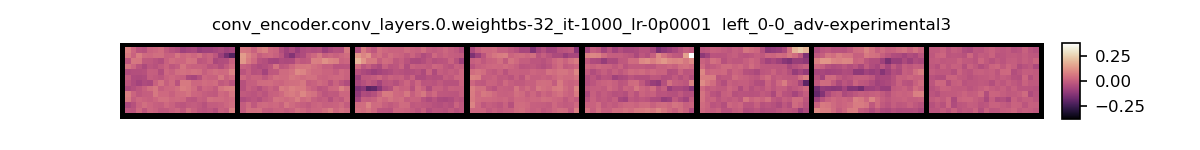
\includegraphics[width=0.45\textwidth]{./3_theory/figs/ml_adv_example_label_left_c0_enc}}
    \subfigure[\enquote{left} c1 from G]{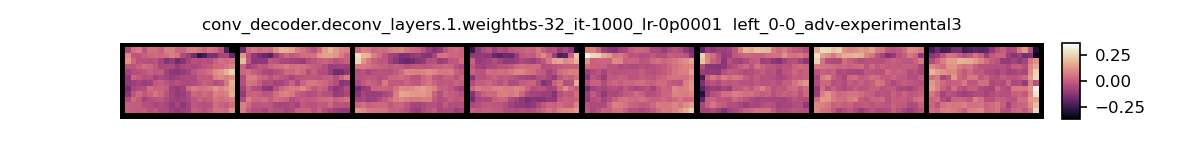
\includegraphics[width=0.45\textwidth]{./3_theory/figs/ml_adv_example_label_left_c0_dec}}
    \subfigure[\enquote{left} c2 from D]{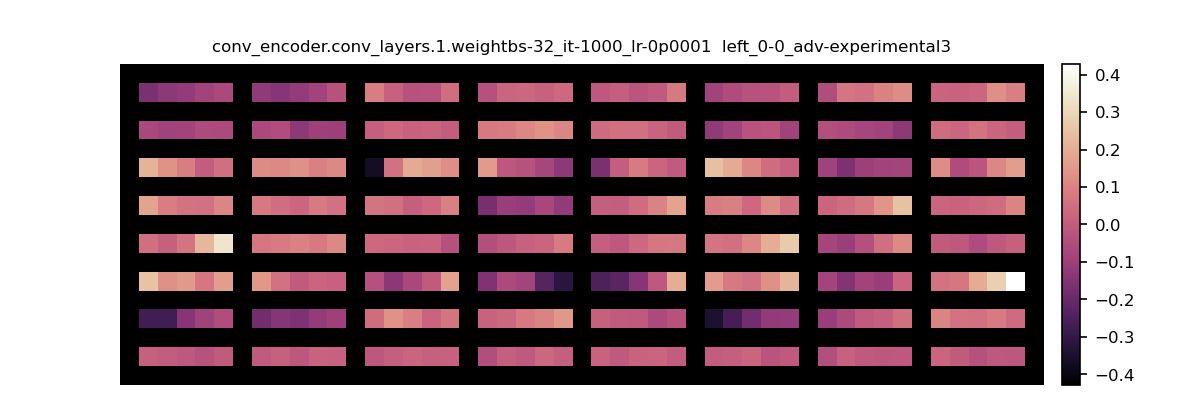
\includegraphics[width=0.3\textwidth]{./3_theory/figs/ml_adv_example_label_left_c1_enc}}
    \subfigure[\enquote{left} c2 from G]{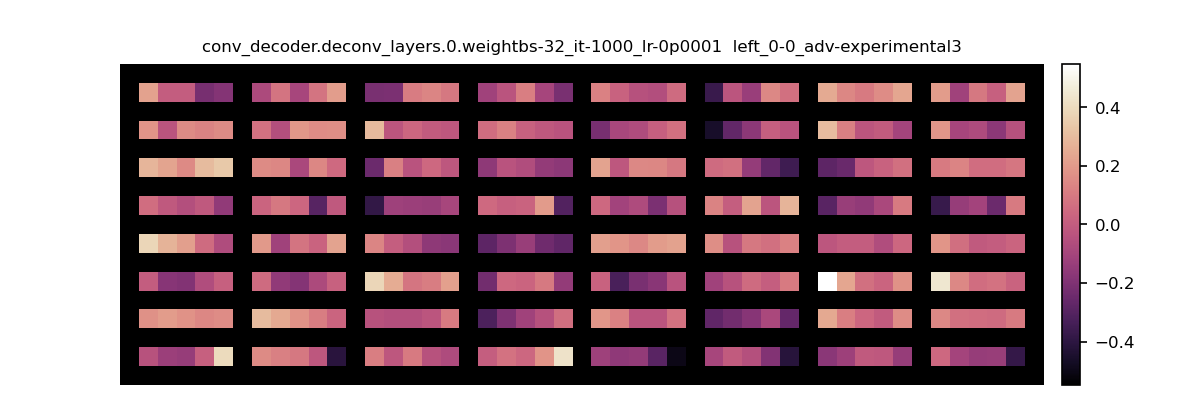
\includegraphics[width=0.3\textwidth]{./3_theory/figs/ml_adv_example_label_left_c1_dec}}
  \caption{Adversarial Training example of Generator (G) and Discriminator (D) of label \enquote{left} captured with 8 feature maps of the first convolutional layer.}
  \label{fig:ml_adv_example_label}
\end{figure}
\FloatBarrier
\noindent

Those trained weights from each label can then simply be put into the feature maps of a classification network.
This is shown in \rfig{ml_adv_example} where c1 from G and c2 from G in \rfig{ml_adv_example_label} were transfered to the first row(s).
When doing the transferring of feature maps, it is important that the layers are not mixed up so that the trained connections are still correct.
Also of course the weights of the feature maps must have the same dimension, so that transferring is possible.


\subsubsection{Observing the Generators output}
While the output of the Discriminator is rather uninteresting (one-dimensional probability value), the output of the Generator is a good indicator of how well the training between D and G has gone.
Optimally the output of the Generator look like real data samples.
An example of a trained Generator Network with fake outputs compared to real ones is shown in \rfig{ml_adv_gen}.

\begin{figure}[!ht]
  \centering
    \subfigure[\enquote{left} real examples]{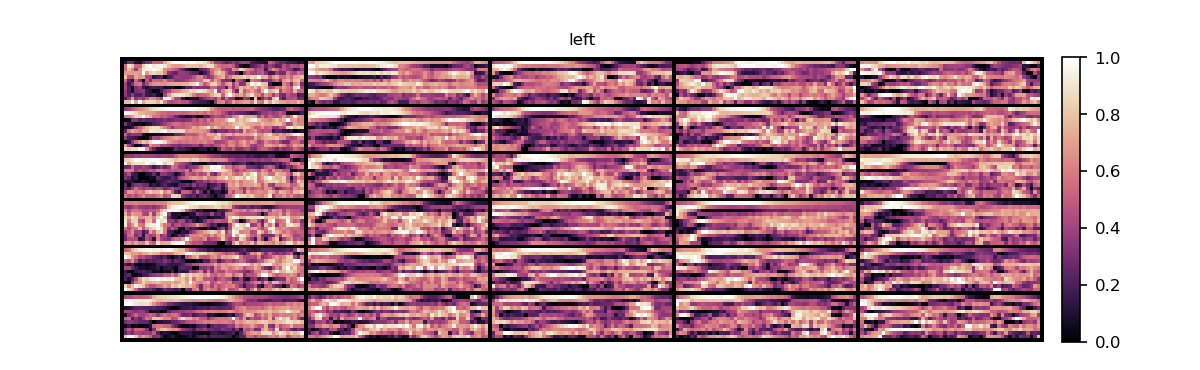
\includegraphics[width=0.45\textwidth]{./3_theory/figs/ml_adv_gen_left_real}}
    \subfigure[\enquote{left} fakes from G]{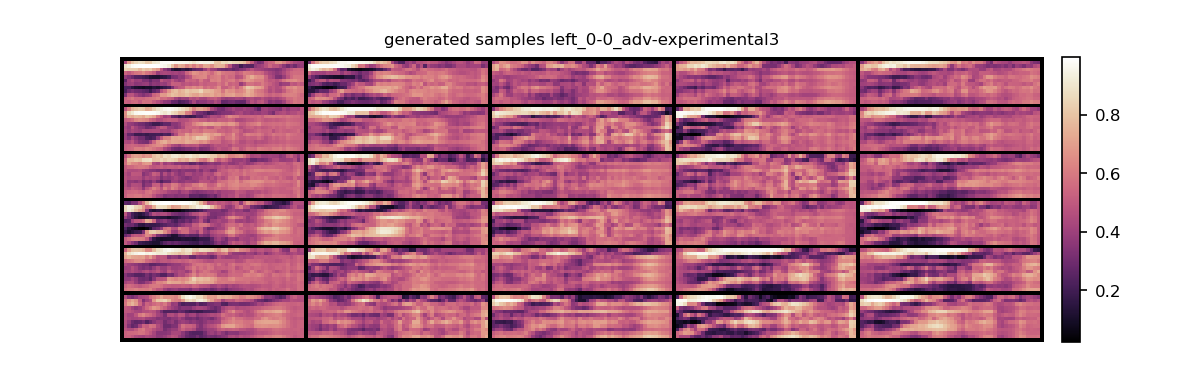
\includegraphics[width=0.45\textwidth]{./3_theory/figs/ml_adv_gen_left_fake}}
  \caption{Real samples of \enquote{left} from the Speech Commands dataset compared to fake samples from a trained Generator Network.}
  \label{fig:ml_adv_gen}
\end{figure}
\FloatBarrier
\noindent

If the fake example of the Generator Network do not look similar to real ones, then something might have gone wrong in the training between the Generator and Discriminator Network.
Further it can be evaluated if a certain network architecture is able to produce a label in a sufficient representation, therefore this method might be a good start in finding a suitable network architecture for the problem to be solved.





% game
\section{Video Game}
Theory?
